\documentclass{ximera}

\author{Anna Davis \and Paul Zachlin} \title{Existence of the Inverse of a Linear Transformation} \license{CC-BY 4.0}

\renewcommand{\vec}[1]{{\bf #1}}
\newcommand{\RR}{\mathbb{R}}
\newcommand{\dfn}{\textit}
\newcommand{\dotp}{\cdot}
\newcommand{\id}{\text{id}}

\newtheorem{general}{Generalization}
\newtheorem{initprob}{Exploration Problem}
\usepackage{tikz-cd}
\usetikzlibrary{shapes.geometric}
\usetikzlibrary{arrows}
\pgfplotsset{compat=1.14}



\begin{document}
\begin{abstract}
  We define  isomorphisms, and prove that a linear transformation has an inverse if and only if the linear transformation is an isomorphism.
\end{abstract}
\maketitle

%Note to Student:  In this module we will often use $U$, $V$ and $W$ to denote the domain and codomain of linear transformations.  If you are familiar with abstract vector spaces, you can regard $U$, $V$ and $W$ as finite-dimensional vector spaces, otherwise you may think of $U$, $V$ and $W$ as subspaces of $\RR^n$. 


\section*{Existence of Inverses}

In Exploration Problem \ref{ep:inverse} of LTR-M-0030 we examined a linear transformation $T:\RR^2\rightarrow \RR^2$ that doubles all input vectors, and its inverse $S:\RR^2\rightarrow \RR^2$, that halves all input vectors.  We observed that the composite functions $S\circ T$ and $T\circ S$ are both identity transformations.  Diagrammatically, we can represent $T$ and $S$ as follows:
 \begin{center}
 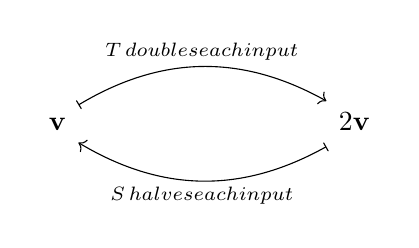
\begin{tikzpicture}
\node{
\begin{tikzcd}[column sep=9em, row sep=huge]
\vec{v} \arrow[r,bend left, "T\,\text{doubles each input}", shift left, mapsto] \arrow[r,bend right, "S\, \text{halves each input}"',shift right, mapsfrom] & 2\vec{v}
\end{tikzcd}
};
\end{tikzpicture}
\end{center}

This gives us a way of thinking about an inverse of $T$ as a transformation that ``undoes" the action of $T$ by ``reversing" the mapping arrows.  We will now use these intuitive ideas to understand which linear transformations are invertible and which are not.

Given an arbitrary linear transformation $T:V\rightarrow W$, ``reversing the arrows"
 may not always result in a transformation. Recall that transformations are functions.  The figures below show two ways in which our attempt to ``reverse" $T$ may fail to produce a function.
 
 First, if two distinct vectors $\vec{v}_1$ and $\vec{v}_2$ map to the same vector $\vec{w}$ in $W$, then reversing the arrows gives us a mapping that is clearly not a function. %(See Figure \ref{fig:notonetoone}) 
 

\begin{center}
\begin{tikzpicture}
\node{
\begin{tikzcd}
\vec{v}_1 \arrow[rd, mapsto]  & \\
& T(\vec{v}_1)=T(\vec{v}_1)=\vec{w}\\
\vec{v}_2 \arrow[ru, mapsto]  &
\end{tikzcd}\quad
\begin{tikzcd}
\vec{v}_1 \arrow[rd, mapsfrom]  & \\
& T(\vec{v}_1)=T(\vec{v}_1)=\vec{w}\\
\vec{v}_2 \arrow[ru, mapsfrom]  &
\end{tikzcd}
};
\end{tikzpicture}
\end{center}
%\caption{One input, $\vec{w}$, produces two outputs, $\vec{v}_1$ and $\vec{v}_2$.}
%  \label{fig:notonetoone} 
  

Second, observe that our definition of an inverse of $T:V\rightarrow W$ requires that the domain of the inverse transformation be $W$. (Definition \ref{def:inverse}, LTR-M-0030)  If there is a vector $\vec{b}$ in $W$ that is not an image of any vector in $V$, then $\vec{b}$ cannot be in the domain of an inverse transformation. %(See Figure \ref{fig:notonto}.)

%\begin{figure}[h]
\begin{center}
\begin{tikzcd}
  & \vec{b} \\
\vec{v} \arrow[r, mapsto] & T(\vec{v})
\end{tikzcd}\quad\quad
\begin{tikzcd}
? \arrow[r, mapsfrom] & \vec{b} \\
\vec{v} \arrow[r, mapsfrom] & T(\vec{v})
\end{tikzcd}\quad
%\caption{$\vec{b}$ is in $W$, but cannot be in the domain of an inverse of $T$.}
  \label{fig:notonto} 
%\end{figure}
\end{center}



We now illustrate these potential issues with specific examples.
\begin{example}\label{ex:notonetoone} Let $T:\RR^2\rightarrow \RR^2$ be a linear transformation whose standard matrix is
$$\begin{bmatrix}1&1\\2&2\end{bmatrix}$$
Does $T$ have an inverse? Show that multiple vectors of the domain map to $\vec{0}$ in the codomain.  

\begin{explanation} The matrix $\begin{bmatrix}1&1\\2&2\end{bmatrix}$ is not invertible, so $T$ does not have an inverse.

We now dig a little deeper to get additional insights into why $T$ does not have an inverse.  Observe that all vectors of the form $\begin{bmatrix}k\\-k\end{bmatrix}$ map to $\vec{0}$.  To verify this, use matrix multiplication:
$$\begin{bmatrix}1&1\\2&2\end{bmatrix}\begin{bmatrix}k\\-k\end{bmatrix}=\begin{bmatrix}0\\0\end{bmatrix}$$
This shows that there are infinitely many vectors that map to $\vec{0}$.  So, ``reversing the arrows" would not result in a function.


\end{explanation}
\end{example}



\begin{example}\label{ex:notonto} Let $T:\RR^2\rightarrow \RR^3$ be a linear transformation whose standard matrix is
$$\begin{bmatrix}1&0\\0&1\\2&0\end{bmatrix}$$
Does $T$ have an inverse? Show that there exists a vector $\vec{b}$ in $\RR^3$ such that no vector of $\RR^2$ maps to $\vec{b}$. 
\begin{explanation}
The matrix $\begin{bmatrix}1&0\\0&1\\2&0\end{bmatrix}$ is not invertible (it's not even a square matrix!), so $T$ does not have an inverse.

We now get another insight into why $T$ is not invertible.
To find a vector $\vec{b}$ such that no vector of $\RR^2$ maps to $\vec{b}$, we need to find $\vec{b}$ for which the matrix equation
\begin{align}\label{ex:matrix}\begin{bmatrix}1&0\\0&1\\2&0\end{bmatrix}\vec{x}=\vec{b}\end{align}
has no solution.  

Let $\vec{b}=\begin{bmatrix}b_1\\b_2\\b_3\end{bmatrix}$.  Gauss-Jordan elimination yields:

$$\left[\begin{array}{cc|c}  
 1 & 0 & b_1\\  
 0 & 1 & b_2\\
 2 & 0 & b_3
\end{array}\right] \rightsquigarrow \left[\begin{array}{cc|c} 
 1 & 0 & b_1\\  
 0 & 1 & b_2\\
 0 & 0 & b_3-2b_1
\end{array}\right]$$
Equation (\ref{ex:matrix}) has a solution if and only if $b_3-2b_1=0$.  Since we do not want (\ref{ex:matrix}) to have a solution, all we need to do is pick values $b_1$, $b_2$ and $b_3$ such that $b_3-2b_1\neq 0$.  Let $\vec{b}=\begin{bmatrix}1\\1\\1\end{bmatrix}$.  Then no element of $\RR^2$ maps to $\vec{b}$.
\end{explanation}
\end{example}

Our next goal is to develop some vocabulary that would allow us to discuss issues illustrated by the figures.

\begin{center}
\begin{tikzpicture}
\node{
\begin{tikzcd}
\vec{v}_1 \arrow[rd, mapsto]  & \\
& T(\vec{v}_1)=T(\vec{v}_1)=\vec{w}\\
\vec{v}_2 \arrow[ru, mapsto]  &
\end{tikzcd}\quad
\begin{tikzcd}
\vec{v}_1 \arrow[rd, mapsfrom]  & \\
& T(\vec{v}_1)=T(\vec{v}_1)=\vec{w}\\
\vec{v}_2 \arrow[ru, mapsfrom]  &
\end{tikzcd}
};
\end{tikzpicture}
\end{center}

\begin{center}
\begin{tikzcd}
  & \vec{b} \\
\vec{v} \arrow[r, mapsto] & T(\vec{v})
\end{tikzcd}\quad\quad
\begin{tikzcd}
? \arrow[r, mapsfrom] & \vec{b} \\
\vec{v} \arrow[r, mapsfrom] & T(\vec{v})
\end{tikzcd}
\end{center}


\subsection*{One-to-one Linear Transformations}

\begin{definition}[One-to-One]\label{def:onetoone} A linear transformation $T:V\rightarrow W$ is one-to-one if 
$$T(\vec{v}_1)=T(\vec{v}_2)\quad \text{implies that}\quad \vec{v}_1=\vec{v}_2$$
\end{definition}

\begin{example}
Transformation $T$ in Example \ref{ex:notonetoone} is not one-to-one.
\begin{explanation}
We can use any two vectors of the form $\begin{bmatrix}k\\-k\end{bmatrix}$ to make our case.  
$$T\left(\begin{bmatrix}1\\-1\end{bmatrix}\right)=\vec{0}=T\left(\begin{bmatrix}-2\\2\end{bmatrix}\right)\quad \text{but}\quad\begin{bmatrix}1\\-1\end{bmatrix}\neq \begin{bmatrix}-2\\2\end{bmatrix}$$
\end{explanation}
\end{example}

\begin{example}
Prove that the transformation in Example \ref{ex:notonto} is one-to-one.
\begin{proof}
Suppose
$$T\left(\begin{bmatrix}x_1\\x_2\end{bmatrix}\right)=T\left(\begin{bmatrix}y_1\\y_2\end{bmatrix}\right)$$
Then
$$\begin{bmatrix}1&0\\0&1\\2&0\end{bmatrix}\begin{bmatrix}x_1\\x_2\end{bmatrix}=\begin{bmatrix}1&0\\0&1\\2&0\end{bmatrix}\begin{bmatrix}y_1\\y_2\end{bmatrix}$$
$$x_1\begin{bmatrix}1\\0\\2\end{bmatrix}+x_2\begin{bmatrix}0\\1\\0\end{bmatrix}=y_1\begin{bmatrix}1\\0\\2\end{bmatrix}+y_2\begin{bmatrix}0\\1\\0\end{bmatrix}$$
$$(x_1-y_1)\begin{bmatrix}1\\0\\2\end{bmatrix}+(x_2-y_2)\begin{bmatrix}0\\1\\0\end{bmatrix}=\vec{0}$$
It is clear that $\begin{bmatrix}1\\0\\2\end{bmatrix}$ and $\begin{bmatrix}0\\1\\0\end{bmatrix}$ are linearly independent.  Therefore, we must have $x_1-y_1=0$ and $x_2-y_2=0$.  But then $x_1=y_1$ and $x_2=y_2$, so 
$$\begin{bmatrix}x_1\\x_2\end{bmatrix}=\begin{bmatrix}y_1\\y_2\end{bmatrix}$$
\end{proof}
\end{example}

At this point we can conjecture that being one-to-one is a necessary, but not a sufficient condition for a linear transformation to have an inverse.  We will consider the other necessary condition next.

\subsection*{``Onto" Linear Transformations}

\begin{definition}[Onto]\label{def:onto} A linear transformation $T:V\rightarrow W$ is onto if for every element $\vec{w}$ of $W$, there exists an element $\vec{v}$ of $V$ such that $T(\vec{v})=\vec{w}$.
\end{definition}

\begin{example}
The transformation in Example \ref{ex:notonto} is not onto.
\begin{explanation}
No element of $\RR^2$ maps to $\begin{bmatrix}1\\1\\1\end{bmatrix}$.
\end{explanation}
\end{example}

\begin{example} Prove that the linear transformation $T:\RR^2\rightarrow \RR^2$ whose standard matrix is $$A=\begin{bmatrix}1&0\\2&1\end{bmatrix}$$ is onto.
\begin{proof} Let $\vec{b}$ be an element of the codomain ($\RR^2$).  We need to find $\vec{x}$ in the domain ($\RR^2$) such that $T(\vec{x})=\vec{b}$. 
Observe that $A$ is invertible, and $$A^{-1}=\begin{bmatrix}1&0\\-2&1\end{bmatrix}$$
 Let $\vec{x}=\begin{bmatrix}1&0\\-2&1\end{bmatrix}\vec{b}$, then 
 $$T(\vec{x})=\begin{bmatrix}1&0\\2&1\end{bmatrix}\left(\begin{bmatrix}1&0\\-2&1\end{bmatrix}\vec{b}\right)=I\vec{b}=\vec{b}$$
\end{proof}
\end{example}

\begin{example}Prove that the linear transformation $T:\RR^3\rightarrow \RR^2$ induced by $$A=\begin{bmatrix}1&1&-1\\2&3&-1\end{bmatrix}$$ is onto.
% \begin{proof} Let $\vec{b}$ be an element of the codomain ($\RR^2$).  We need to find $\vec{x}$ in the domain ($\RR^3$) such that $T(\vec{x})=\vec{b}$.   To do this we will solve the equation
% $$\begin{bmatrix}1&1&-1\\2&3&-1\end{bmatrix}\vec{x}=\vec{b}$$
% Let $\vec{b}=\begin{bmatrix}b_1\\b_2\end{bmatrix}$. Gauss-Jordan elimination yields:

% {\color{red}(Paul, I don't know why I made the rest of it so specific, we could just claim that there are infinitely many solutions for whatever b we choose.  Is the specificity helpful to students?  Sometimes it's nice to know that not only does the thing exist, but you can actually find it.)}

% $$\left[\begin{array}{ccc|c}  
%  1 & 1 & -1 & b_1\\  
%  2 & 3 & -1 & b_2
% \end{array}\right] \rightsquigarrow \left[\begin{array}{ccc|c} 
%  1 & 0 & -2 & 3b_1-b_2\\  
%  0 & 1 & 1 & b_2-2b_1
% \end{array}\right]$$
% There are infinitely many solution, but we only need to find one.  
% Let $\vec{x}=\begin{bmatrix}3b_1-b_2\\ b_2-2b_1\\0\end{bmatrix}$.  Then
% $$T(\vec{x})=\begin{bmatrix}1&1&-1\\2&3&-1\end{bmatrix}\begin{bmatrix}3b_1-b_2\\ b_2-2b_1\\0\end{bmatrix}=\begin{bmatrix}b_1\\b_2\end{bmatrix}=\vec{b}$$
% \end{proof}

\begin{proof}

Let $\vec{b}$ be an element of $\RR^2$.  We need to show that there exists $\vec{x}$ in $\RR^3$ such that $T(\vec{x})=A\vec{x}=\vec{b}$. 
Observe that
 $$\textnormal{rref}(A)=\begin{bmatrix}1 & 0 & -2\\0 & 1 & 1\end{bmatrix}$$
 This means that $A\vec{x}=\vec{b}$ has a solution (in fact, it has infinitely many solutions).  Therefore $\vec{b}$ is an image of some $\vec{x}$ in $\RR^3$. We conclude that $T$ is onto. 
 
 


% The two rows of $A$ are clearly linearly independent.  Therefore $rank(A)=2$.  We know $col(A)$ is a subspace of $\RR^2$ {\color{red} reference?}, and since $\text{dim}(\text{col}(A))=\text{rank}(A)=2$, it suffices to take two linearly independent columns as a basis for $col(A)$.  If we take the first two columns of $A$ to be our basis, it is easy to see that any vector $\vec{v} \in \RR^2$ can be written as a linear combination of those columns (do you remember how?):
% $$\vec{v}= a \begin{bmatrix}1\\2\end{bmatrix} + b \begin{bmatrix}1\\3\end{bmatrix} $$
% But since $T(\vec{i})=\begin{bmatrix}1\\2\end{bmatrix}$ and $T(\vec{j})=\begin{bmatrix}1\\3\end{bmatrix}$, we can also write
% $$\vec{v}= T(a \vec{i} + b \vec{j}) .$$
% {\color{red} is it better to use $\vec{e_1}$ and $\vec{e_2}$ instead of $\vec{i}$ and $\vec{j}$?}{\color{blue} I am neutral on this question, but I've been using i, j, k when talking about $R^2$ and $R^3$, so I would have to go back and redo a bunch of stuff if we switch.}
\end{proof}
\end{example}

\section*{Isomorphisms and Existence of Inverses}

\begin{definition} A linear transformation that is one-to-one and onto is called an isomorphism.
\end{definition}

\begin{example}\label{ex:subtosub} Let $$V=\text{span}\left(\begin{bmatrix}1\\0\\0\end{bmatrix}, \begin{bmatrix}1\\1\\1\end{bmatrix}\right)$$
Define a linear transformation $$T:V\rightarrow \RR^2$$
by $$T\left(\begin{bmatrix}1\\0\\0\end{bmatrix}\right)=\begin{bmatrix}1\\1\end{bmatrix}\quad \text{and} \quad T\left(\begin{bmatrix}1\\1\\1\end{bmatrix}\right)=\begin{bmatrix}0\\1\end{bmatrix}$$
%(Why is it sufficient to specify the images of $\begin{bmatrix}1\\0\\0\end{bmatrix}, \begin{bmatrix}1\\1\\1\end{bmatrix}$ to define this linear transformation?)  
Show that $T$ is an isomorphism.
\begin{proof}

We will first show that $T$ is one-to-one.  
Suppose 
$$T(\vec{u})=T(\vec{v})$$
for some $\vec{u}$ and $\vec{v}$ in $V$. Vectors $\vec{u}$ and $\vec{v}$ are in the span of $\begin{bmatrix}1\\0\\0\end{bmatrix}$ and $\begin{bmatrix}1\\1\\1\end{bmatrix}$, so

$$\vec{u}=a\begin{bmatrix}1\\0\\0\end{bmatrix}+b\begin{bmatrix}1\\1\\1\end{bmatrix}\quad\text{and}\quad \vec{v}=c\begin{bmatrix}1\\0\\0\end{bmatrix}+d\begin{bmatrix}1\\1\\1\end{bmatrix}$$
for some scalars $a, b, c, d$.

$$T(\vec{u})=aT\left(\begin{bmatrix}1\\0\\0\end{bmatrix}\right)+bT\left(\begin{bmatrix}1\\1\\1\end{bmatrix}\right)=a\begin{bmatrix}1\\1\end{bmatrix}+b\begin{bmatrix}0\\1\end{bmatrix}=\begin{bmatrix}a\\a+b\end{bmatrix}$$

$$T(\vec{v})=cT\left(\begin{bmatrix}1\\0\\0\end{bmatrix}\right)+dT\left(\begin{bmatrix}1\\1\\1\end{bmatrix}\right)=c\begin{bmatrix}1\\1\end{bmatrix}+d\begin{bmatrix}0\\1\end{bmatrix}=\begin{bmatrix}c\\c+d\end{bmatrix}$$
Thus,
$$\begin{bmatrix}a\\a+b\end{bmatrix}=\begin{bmatrix}c\\c+d\end{bmatrix}$$
This implies that $a=c$ which, in turn, implies $b=d$.  This gives us $\vec{u}=\vec{v}$, and we conclude that $T$ is one-to-one.

Next we will show that $T$ is onto.  

The key observation is that vectors $\begin{bmatrix}1\\1\end{bmatrix}$ and $\begin{bmatrix}0\\1\end{bmatrix}$ span $\RR^2$.  Perhaps this is easiest seen by noting that $$\text{rank}\left(\begin{bmatrix}1&0\\1&1\end{bmatrix}\right)=2$$

This means that given a vector $\vec{v}$ in $\RR^2$, we can write $\vec{v}$ as $\vec{v}=a\begin{bmatrix}1\\1\end{bmatrix}+b\begin{bmatrix}0\\1\end{bmatrix}$.  But this means that $\vec{v}=T\left(a\begin{bmatrix}1\\0\\0\end{bmatrix}+b\begin{bmatrix}1\\1\\1\end{bmatrix}\right)$  We conclude that $T$ is onto. 

Since $T$ is a linear transformation that  is one-to-one and onto, $T$ is an isomorphism.
\end{proof}
\end{example}

\begin{theorem}\label{th:isomeansinvert} Let $V$ and $W$ be vector spaces, and let $T:V\rightarrow W$ be a linear transformation.  Then $T$ has an inverse if and only if $T$ is an isomorphism. 
\end{theorem}
\begin{proof}
We will first assume that $T$ is an isomorphism and show that there exists a transformation $S:W\rightarrow V$ such that $S\circ T=\id_V$ and $T\circ S=\id_W$.  Because $T$ is onto, for every $\vec{w}$ in $W$, there exists $\vec{v}$ in $V$ such that $T(\vec{v})=\vec{w}$.  Moreover, because $T$ is one-to-one, vector $\vec{v}$ is the only vector that maps to $\vec{w}$.  To stress this, we will say that for every $\vec{w}$, there exists $\vec{v}_{\vec{w}}$ such that $T(\vec{v}_{\vec{w}})=\vec{w}$. (Since every $\vec{v}$ maps to exactly one $\vec{w}$, this notation makes sense for elements of $V$ as well.)  We can now define $S:W\rightarrow V$ by $S(\vec{w})=\vec{v}_{\vec{w}}$.
Then
$$(S\circ T)(\vec{v}_{\vec{w}})=S(T(\vec{v}_{\vec{w}}))=S(\vec{w})=\vec{v}_{\vec{w}}$$
$$(T\circ S)(\vec{w})=T(S(\vec{w}))=T(\vec{v}_{\vec{w}})=\vec{w}$$
We conclude that $S\circ T=\id_V$ and $T\circ S=\id_W$.  Therefore $S$ is an inverse of $T$.

We will now assume that $T$ has an inverse $S$ and show that $T$ must be an isomorphism.  To show that $T$ is an isomorphism, we need to show that $T$ is one-to-one and onto.
Suppose $$T(\vec{v}_1)=T(\vec{v}_2)$$ then $$S(T(\vec{v}_1))=S(T(\vec{v}_2))$$
but then
$$\vec{v}_1=\vec{v}_2$$
We conclude that $T$ is one-to-one.

Now suppose that $\vec{w}$ is in $W$.  We need to show that some element of $V$ maps to $\vec{w}$.  Let $\vec{v}=S(\vec{w})$.  Then
$$T(\vec{v})=T(S(\vec{w}))=(T\circ S)(\vec{w})=\id_W(\vec{w})=\vec{w}$$
We conclude that $T$ is onto.
\end{proof}

\begin{example}\label{ex:subtosubinvert}
Transformation $T$ in Example \ref{ex:subtosub} is invertible.
\begin{explanation}
We demonstrated that $T$ is an isomorphism.  By Theorem \ref{th:isomeansinvert}, $T$ has an inverse.  

Recall that $T$ was introduced in Exploration Problem \ref {init:subtosub} of LTR-M-0030 to demonstrate that Theorem \ref{th:existunique} of LTR-M-0030 is not always applicable.  We now have additional tools. Theorem \ref{th:isomeansinvert} assures us that $T$ has an inverse, but does not help us find it. We will visit this problem again, in LTR-M-0080, and find an inverse of $T$.
\end{explanation}
\end{example}

\subsection*{Uniqueness of Inverses}

Definition \ref{def:inverse} of LTR-M-0030 refers to $S$ as \dfn{an} inverse of $T$, implying that there may be more than one such transformation $S$.  We will now show that if such a transformation $S$ exists, it is unique.  This will allow us to refer to {\it the} inverse of $T$ and to start using $T^{-1}$ to denote the unique inverse of $T$.

\begin{theorem}\label{th:inverseisunique}
If $T$ is a linear transformation, and $S$ is an inverse of $T$.  Then $S$ is unique.
\end{theorem}
\begin{proof}
Let $T:V\rightarrow W$ be a linear transformation.  If $S$ is an inverse of $T$, then $S$ satisfies
$$S\circ T=\id_V\quad \text{and}\quad T\circ S=\id_W$$

Suppose there is another transformation, $S'$, such that 
$$S'\circ T=\id_V\quad \text{and}\quad T\circ S'=\id_W$$
We now show that $S=S'$.
$$S=S\circ \id_W=S\circ(T\circ S')=(S\circ T)\circ S'=\id_V\circ S'=S'$$
\end{proof}

\section*{Practice Problems}
\begin{problem}
Show that a linear transformation $T:\RR^2\rightarrow \RR^2$ with standard matrix $A=\begin{bmatrix}2&-4\\-3&6\end{bmatrix}$ is not one-to-one.
\begin{hint}
        Show that multiple vectors map to $\vec{0}$.
      \end{hint}
\end{problem}
 
 \begin{problem}
 Show that a linear transformation $T:\RR^2\rightarrow \RR^3$ with standard matrix $A=\begin{bmatrix}1&2\\-1&1\\0&1\end{bmatrix}$ is not onto.
 \begin{hint}
 Find $\vec{b}$ such that $A\vec{x}=\vec{b}$ has no solutions.
 \end{hint}
 \end{problem}
 
 \begin{problem}
 Suppose that a linear transformation $T:\RR^3\rightarrow \RR^3$ has a standard matrix $A$ such that $\text{rref}(A)=I$.
 
 Prove that $T$ is one-to-one.
 \begin{hint}
 How many solutions does $A\vec{x}=\vec{b}$ have?
 \end{hint}
 Prove that $T$ is onto.
 \begin{hint}
 Does $A\vec{x}=\vec{b}$ have a solution for every $\vec{b}$?
 \end{hint}
 \end{problem}
 
 \begin{problem}
 Define a transformation $T:\RR^2\rightarrow \RR^2$ by 
 $$T\left(\begin{bmatrix}x\\y\end{bmatrix}\right)=\begin{bmatrix}x\\-2x+4y\end{bmatrix}$$
 Show that $T$ is an isomorphism.
 \begin{hint}
 Don't forget to show that $T$ is linear.
 \end{hint}
 \end{problem}
 
 \begin{problem}
 Let $V=\text{span}\left(\begin{bmatrix}1\\0\\1\end{bmatrix}, \begin{bmatrix}0\\1\\0\end{bmatrix}\right)$.  Define a linear transformation $T:V\rightarrow \RR^2$ by
 $$T\left(\begin{bmatrix}1\\0\\1\end{bmatrix}\right)=\begin{bmatrix}0\\1\end{bmatrix}\quad \text{and}\quad T\left(\begin{bmatrix}0\\1\\0\end{bmatrix}\right)=\begin{bmatrix}-1\\1\end{bmatrix}$$
 Prove that $T$ is an isomorphism.
 \end{problem}
\end{document}
